\chapter{} 
\pagenumbering{arabic} % 阿拉伯数字页码

\section{研究目的}
计算机视觉中多标签分类(Multi-label)问题可以看做是多类别(Multi-class)问题的泛化,
多标签分类将一个实例分到多个类别中去.
\subsection{研究背景}

随着移动互联网时代的到来,图像数据与日俱增,这就造就了图像大数据时代的到来,
传统的图像单标签分类问题已经无法满足含有复杂语义图像的分类识别要求,这时候就需要分类识别
速度快,精度高的多标签图像分类技术,该技术的出现推动了图像大数据时代的发展。
关于多标签分类技术,一般过程是这样的:假如有了训练集(用于训练的图片)及测试
集(用来测试的图片),首先提取训练集中的有标签图片,添加多层神经网络训练这些图片
,得到训练模型,最后用训练模型检验测试集,来测试模型识别的精准度。这样的话,
通常需要很大的测试集和训练次数,至少要有10000张测试图片、10000次最大训练次数,
才能得到一个较好的图片识别精准度,如果我们按照上述的步骤来完成我们的多标签分类的研究,
这样做的意义并不大:一是这样需要非常大的电脑计算能力和计算开销,我们的机器难以达到这种要求;
二是就算我们的电脑能支持这种开销,最终得到训练模型,别人完全可以单
纯的通过增加测试图片和增加训练次数来超过我们的模型识别图像的精准度,且Google已经提供了不少
花费了几十甚至数百个GPU小时的训练模型,那么这样我们的研究工作就没什么意义了。所以我们工作便放在了
另一个方面上,可以这么想:你的训练图片和训练次数越多,你的图像识别精度越高,然而达到了一个较高的
上限后,无论你再怎么添加训练图片和训练次数,你的图像识别精度就难以提升了,这时怎么提高精度呢?这
便是我们所要研究的工作,我们用到了深度学习之——迁移学习,通过使用已有的预训练模型,提取其中神
经网络中信息的权重,迁移到我们神经网络,我们学习了这些特征,然后通过再训练来修正完善这些特征,便
在已有的训练模型的基础上提高了图像识别的精准率,这样我们的研究变具有了价值性。我们工作的重点在于预训练
模型中找到能够输出可复用特征(feature)的层次(layer),然后利用该层次的输出作为输入特征来训练那些需要
参数较少的规模更小的神经网络.

\subsection{研究意义}

随着照片和视频分享网站的普及(Flicker,Instagram和Youtube等等),大量的未标记的和弱标记的图像数据也随着传播开来。这越来越多的数据图像需要有效的数据检索来达到获取这个图像的最终目的。尽管图像检索已经被研究许多年了,搜索引擎检索目的图像仍然大多基于文本内容而非原始图像语义。因此,自动将图像标注成人类已经提供好的关键词或者标签的技术已经受到了大量的研究关注。
该技术从开始到现在的发展大致经历了三个阶段,分别是:基于文本的图像检索,基于内容的图像检索,基于语义的图像检索。基于文本的图像检索,由于手工标注工作量大,个人理解也有差异,导致检索结果出错率较高;基于内容的图像检索,是根据图像的底层特征进行检索,没有反映图像的内容信息;而基于语义的图像检索,弥补了上述两种方法的缺陷,使检索结果和使用者所需要的信息尽可能的一致。
对于语义标注可以人工标注或者机器标注,由于上述所讲个人的理解因人而异,所以现在大多使用机器自动标注,即将等待标注的图像输入计算机系统,经过分割,将它划为等大的方格,而每个小方格的特征都被一个视觉特征词代替,让系统通过一系列算法推理出可能划分的语义,并将整个图像转为语义序列,相邻而重复的视觉词去掉然后将每个视觉词标注它所对应的物体标签。


\subsection{研究目的}

以多标签图像标注为目的,在Keras深度学习框架下,使用Python语言,结合TensorFlow库,开发图像标注的核心算法。结合ResNet50预训练模型和以上算法训练出属于我们自己的模型,在预训练模型的基础上提高其泛化能力及其图片识别的精准率,最后实现对图片的多标签分类。
\section{Multi-label问题简介}

计算机视觉中分类问题是一个重要课题,图像分类有两类问题:一是多分类(multi-class)问题,二是多标签(multi-label)分类问题.
我们要研究的是multi-label classification问题,在多标签分类中,一个实例可以对应多个标签.比如,一张山水画就对应'山'和
'水'或更多标签.多标签分类问题可以看做是多分类问题的泛化,解决起来要比多分类问题困难很多.


\section{研究方法}

我们确定以机器学习中的深度学习模式来进行我们的研究。工具上采用Tensorflow和Keras这两个神经网络库。其中Tensorflow是谷歌官方开源的通用深度学习系统,
而Keras则进行了更高层的封装,现已成为谷歌Tensorflow的默认API

\subsection{开发工具}
我们的技术路线是Tensorflow+keras+Kaggle
\paragraph{TensorFlow介绍}
TensorFlow是谷歌基于DistBelief进行研发的第二代人工智能学习系统,其命名来源于本身的运行原理。Tensor(张量)意味着N维数组,Flow(流)意味着基于数据流图的计算,TensorFlow为张量从流图的一端流动到另一端计算过程。TensorFlow是将复杂的数据结构传输至人工智能神经网中进行分析和处理过程的系统TensorFlow可被用于语音识别或图像识别等多项机器学习和深度学习领域,且完全开源,任何人都可以用。
TensorFlow作为一个机器学习库能做很多事情:

\begin{itemize}
    \item 可自行设计神经网络结构;
    \item 不需要通过反向传播求解梯度,Tensorflow支持自动求导;
    \item 通过C++编写核心代码,简化了线上部署的复杂度(通过SWIG实现Python,Go和JAVA接口);
    \item 谷歌的Tensorflow中内置TF.Learn和TF.Slim等组件,并兼容Sciket-learn estimator接口(evaluate、grid、search、cross、validation);
    \item 数据流式图支持自由的算法表达,可实现深度学习以外的机器学习算法;
    \item 可写内层循环代码控制计算图分支的计算,可将相关的分支转化为子图并执行迭代计算;
    \item 可进行并行设计,充分利用硬件资源。 
    \item 具有灵活的移植性,编译速度较快;
    \item 在数据并行模式上:Tensorflow主要面向内存足以装载模型参数环境,从而实现计算效率的最大化;
    \item 支持卷积神经网络(Convolutional Neural Network ,CNN),循环神经网络(Recurrent Neural Network,RNN),支持深度强化学习及计算密集的科学计算(偏微分方程求解);
\end{itemize}

\paragraph{Keras介绍}
Keras是一个高层神经网络API,Keras由纯Python编写而成并基Tensorflow、Theano以及CNTK后端。Keras 为支持快速实验而生,能够把你的idea迅速转换为结果,Keras的特点:

\begin{itemize}
    \item 简易和快速的原型设计(keras具有高度模块化,极简,和可扩充特性)
    \item 支持CNN和RNN,或二者的结合
    \item 用户友好:Keras是基于TensorFlow。用户的使用体验始终是它的中心内容。Keras遵循减少认知困难的最佳实践:Keras提供一致而简洁的API, 能够极大减少一般应用下用户的工作量,同时,Keras提供清晰和具有实践意义的bug反馈。
    \item 模块性:模型可理解为一个层的序列或数据的运算图,完全可配置的模块可以用最少的代价自由组合在一起。具体而言,网络层、损失函数、优化器、初始化策略、激活函数、正则化方法都是独立的模块,你可以使用它们来构建自己的模型。
    \item 易扩展性:添加新模块超级容易,只需要仿照现有的模块编写新的类或函数即可。创建新模块的便利性使得Keras更适合于先进的研究工作。
    \item 与Python协作:Keras没有单独的模型配置文件类型(作为对比,caffe有),模型由python代码描述,使其更紧凑和更易debug,并提供了扩展的便利性。
\end{itemize}

\paragraph{Kaggle平台介绍}

Kaggle主要为开发商和数据科学家提供举办机器学习竞赛、托管数据库、编写和分享代码的平台。
该平台已经吸引了80万名数据科学家的关注.Kaggle提供了优秀的云编程的环境,还可以免费
使用其服务器,达到在云上训练神经网络模型的目的.我们的电脑配置都比较差,学校也没有给我们
提供计算的服务器,经费远远不够租用AWS服务器,给我们做实验和编写代码带来极大困难.
采用Kaggle平台虽然计算资源还是比较有限,但略微改善了我们的实验环境.
而且Kaggle用docker部署,用到的tensorflow、Keras等库基本上都预装好,
使我们免除配置环境的麻烦.


\subsection{迁移学习}

\subsubsection{什么是迁移学习}

迁移学习(Transfer learning) 顾名思义就是就是把已学训练好的模型参数迁移到新的模型来帮助新模型训练。
考虑到大部分数据或任务是存在相关性的,所以通过迁移学习我们可以将已经学到的模型参数(也可理解为模型学到的知识)
通过某种方式来分享给新模型从而加快并优化模型的学习效率不用像大多数网络那样从零学习。

迁移学习的基本思路是利用预训练模型,即已经通过现成的数据集训练好的模型(这里预训练的数据集可以对应完全不同
的待解问题,例如具有相同的输入,不同的输出)。开发者需要在预训练模型中找到能够输出可复用特征(feature)的
层次(layer),然后利用该层次的输出作为输入特征来训练那些需要参数较少的规模更小的神经网络。
由于预训练模型此前已经习得了数据的组织模式(patterns),因此这个较小规模的网络只需要学习数据中针对特定问题
的特定联系就可以了。

\subsubsection{迁移学习的一般过程}

一般的迁移学习过程是这样的:训练好一个网络(我们称它为base network)→把它的前n层复制到
target network的前n层→target network剩下的其他层随机初始化→开始训练target task。
其中,在做backpropogate(反向传播)的时候,有两种方法可以选择:(1)把迁移过来的这
前n层frozen(冻结)起来,即在训练target task的时候,不改变这n层的值;
(2)不冻结这前n层,而是会不断调整它们的值,称为fine-tune(微调)。这个
主要取决于target数据集的大小和前n层的参数个数,如果target数据集很小,
而参数个数很多,为了防止overfitting(过拟合),通常采用frozen方法;反之,采用fine-tune。

\subsection{预训练模型}
预训练模型(pretrained model):预训练模型是指前人为了解决某类问题所建立的模型。
而当我们为了解决这种类似问题而借用这种模型,这种模型就称为预训练模型。
有了这个预训练模型,在我们解决这类问题的时候,我们可以借鉴前人的经验开始
训练一个模型而不是从头开始为这个问题建立模型并且训练它。
模型信息:
如图~\ref{pre-trained models}所示.
\begin{figure}[!htbp]
	\centering	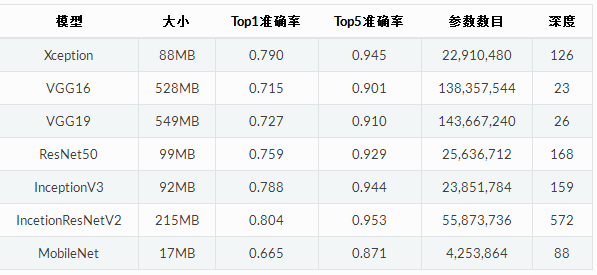
\includegraphics[width=12cm]{pic/assets/premodels}
    \caption{pre-trained models}	\label{pre-trained models}	\end{figure}

我们用预训练模型是ResNet50,
    ResNet50函数原型
\begin{minted}{python}
    keras.applications.resnet50.ResNet50(include_top=True, weights='imagenet',
                                    input_tensor=None, input_shape=None,
                                    pooling=None,
                                    classes=1000)
\end{minted}

    50层残差网络模型,权重训练自ImageNet
    该模型在Theano和TensorFlow后端均可使用,并接受channels\_first和channels\_last两种输入维度顺序
    模型的默认输入尺寸时224x224. 参数如下
    \begin{itemize}

        \item  include\_top:是否保留顶层的全连接网络
        \item  weights:None代表随机初始化,即不加载预训练权重。'imagenet'代表加载预训练权重
        \item  input\_tensor:可填入Keras tensor作为模型的图像输出tensor
        \item  input\_shape:可选,仅当include\_top=False有效,应为长为3的tuple,指明输入图片的shape,图片的宽高必须大于197,如(200,200,3)
        \item  pooling:当include\_top=False时,该参数指定了池化方式。None代表不池化,最后一个卷积层的输出为4D张量。‘avg’代表全局平均池化,‘max’代表全局最大值池化。
        \item  classes:可选,图片分类的类别数,仅当include\_top=True并且不加载预训练权重时可用。
    \end{itemize}

\subsection{基本概念}
% 公式如图~\ref{sigmoid1}所示.
% \begin{figure}[!htbp]
% 	\centering	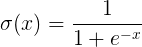
\includegraphics[width=6cm]{pic/assets/sigmoidfuc}
%     \caption{sigmoid激活函数公式}	\label{sigmoid1}	\end{figure}

% 图像如图~\ref{sigmoid2}所示.
% \begin{figure}[!htbp]
% 	\centering	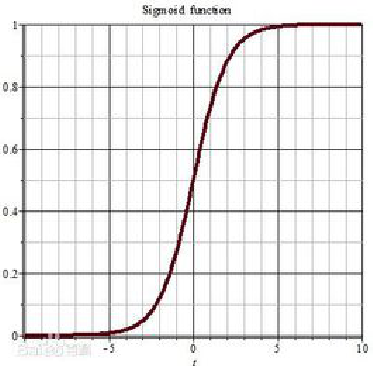
\includegraphics[width=6cm]{pic/assets/sigmoidpic}
%     \caption{sigmoid激活函数图像}	\label{sigmoid2}	\end{figure}

\subsubsection{激活函数}

\begin{figure}[!htbp]
	\centering	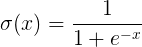
\includegraphics[width=2cm]{pic/assets/sigmoidfuc}
    \caption{sigmoid函数}	\label{sigmoid}	\end{figure}

激活函数(activation function):运行时激活神经网络中某一部分神经元,将激活信息向后传入下一层的神经网络。
神经网络之所以能解决非线性问题(如语音、图像识别),本质上就是激活函数加入了非线性因素,弥补了线性模型的表达力,
把“激活的神经元的特征”通过函数保留并映射到下一层。
这里我们使用的是sigmoid函数。这是传统神经网络中最常用的激活函数之一(另一个是tanh)对应的公式和图像.

\paragraph{sigmoid}

\begin{figure}[!htbp]
    	\centering	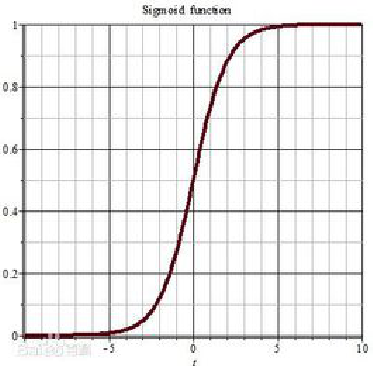
\includegraphics[width=3cm]{pic/assets/sigmoidpic}
        \caption{sigmoid函数图像}	\label{sigmoidpic}	\end{figure}
    

Sigmoid函数的优点在于,它的输出映射在(0,1)内,单调连续,非常适合用作输出层,
并且求导比较容易。但是,它也有缺点,因为软饱和性,一旦落入饱和区,导数就会变得接近于0,
很容易产生梯度消失。
% 维基百科上对softmax的介绍
% In mathematics, the softmax function, or normalized exponential 
% function,is a generalization of the logistic function 
% that "squashes" a K-dimensional vector of arbitrary real values 
% to a K-dimensional vector of real values, where each entry is in 
% the range (0, 1), and all the entries adds up to 1. The function 
% is given by pic~\ref{softmax1}
% \begin{figure}[!htbp]
% 	\centering	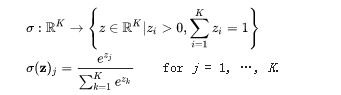
\includegraphics[width=12cm]{pic/assets/softmax1}
%     \caption{softmax1}	\label{softmax1}	\end{figure}


\section{Resnet简单原理}

Resnet要解决的大概是这样的问题:神经网络越来越深的时候,反传回来的梯度之间的相关性会越来越差,最后接近白噪声。
因为我们知道图像是具备局部相关性的,那其实可以认为梯度也应该具备类似的相关性,这样更新的梯度才有意义,如果梯度
接近白噪声,那梯度更新可能根本就是在做随机扰动。

有了梯度相关性这个指标之后,作者分析了一系列的结构和激活函数,发现resnet在保持梯度相关性方面很优秀。
这一点其实也很好理解,从梯度流来看,有一路梯度是保持原样不动地往回传,这部分的相关性是非常强的。

resnet的提出就是为了解决网络加深时的训练精度下降问题, 也被作者称之为退化问题。

\subsection{实验过程}
\subsubsection{数据的预处理}

数据的预处理在机器学习中往往被忽略,其实它很重要,并且不容易做好。

\paragraph{数据集的确定}

首先确定数据集,数据集的选取决定了最终训练效果的上限,如果数据集质量不错的情况下,
那数据当然多多益善。我们的多标签图像分类任务中,可以选择著名的ImageNet
、MS COCO数据集或者更大的OpenImage,我们前期也试图去使用。
深度学习很重要的一个要求是大量的计算资源和充足的经费,
然而作为普通的本科学生,学校提供的活动经费和我们可用的计算资源实在
是太微不足道了,完全不能在这些数据集上完成训练任务。

Multi-label问题中的数据集很多,但绝大多数都不适用于我们经费和计算
资源极其有限的现实情况,因此找到一个大小对我们合适,而又符合我们研究目的的数据
集是很困难的。我们先后尝试了很多,最后确定了南京大学周志华教授LAMDA组公开的多
示例多标签数据集miml-image-data,数据集由2000张自然风景图片和标签组成:
图片的内容有山、水、日落、海、树这五类组成,其中每个图片内容包含一类或多类;
图片对应的标签在.mat格式的文件中给出。.mat是Matlab的文件格式,
这个文件中有数据集的几个属性,有target等属性,图片标签由
[-1,1,-1,-1,1]这种形式给出,依次对应那五类,-1则代表没有,1代表图片有这个标签。
整个数据集压缩后大小为28MB.

\paragraph{数据的清洗与读入}

南大提供的数据集应该还是比较干净的,数据的清洗基本上只要统一大小。
原始图片和.mat的标签并不利于模型的读入,利用tensorflow和之上的keras做开发时
把它们处理后保存为tensorflow的结构化数据格式是比较理想的方式,
这样可以更高效和方便地加载数据。为了提高预测效果和增强模型的泛化能力,我们在此转化的
过程中还做了数据的增广(data augmentation),将其中的图片改变大小和剪裁等,因此转化
后的数据比原始数据大几倍.

\subsubsection{预训练模型的加载}

预训练模型采用Resnet50模型,Resnet由何恺明提出,意为深度残差网络,
在kaggle网站上可以下载到很多预训练模型,这里使用Resnet50,
下载到.h5文件将它放在.keras模型配置文件夹.keras/models中。

\paragraph{为什么要使用预训练模型?}

Google为在Imagenet上训练神经网络,使用了很多GPU,连续训练了几周,
使用了大数据和大量计算资源,这些预训练好的模型可以看做以二进制存放的智慧.
作为普通本科生,学校提供给我们的项目经费和计算资源极其有限,
若不使用预训练模型,不可能达到有意义的训练效果。
而且当数据集也极其有限的时候,预训练模型显得更加必要。

使用预训练模型将给模型的训练一个很好的起点,最终也往往也取得比直接在目标数据集从0开始的训练更好的效果。

\paragraph{模型预测层的再建立}

预训练模型大体由两部分组成,一是抽取特征的部分,二是用于预测的部分。迁移学习有一定的适用条件,
预训练的模型在现实场景的ImageNet数据集上训练,我们自己使用的模型也是现实的自然风景,
因此是符合迁移学习的适用条件的。预训练模型使用了大量的计算资源,
有效地学习到了抽取的图像特征,这是宝贵的经验,应当留下来。我们的计算资源和经费极其有限,
数据集的规模也很小,预训练模型学习到的特征应当尽可能多地保留下来。

有了预训练模型,我们的起点就比较高,因此学习速率(learning rate)应当调小,
否则将很快将之前在大数据训练中得到的合适权重带偏,然后在小数据集上很快陷入
过拟合状态,预测效果反而下降。因此训练过程中应当把预训练模型的前面很多层的
权重都冻结,我们可以训练预训练模型的最后几层,或者自己再在预训练模型除预测部
分的特征提取的最后加上自己建立的卷积层、池化层等,在我们的小数据集训练。
通过反向传播调整特征提取部分最后几层的权重,
这样就达到了既不扰乱预训练模型训练得到的大部分合适权重,
又能有针对性地在我们的小数据集上训练和强化的效果。这样我们就能通过小型数据集,利用
极其有限的计算资源取得理想的训练效果。

如图~\ref{VGG模型}~所示。
\begin{figure}[!htbp]
	\centering	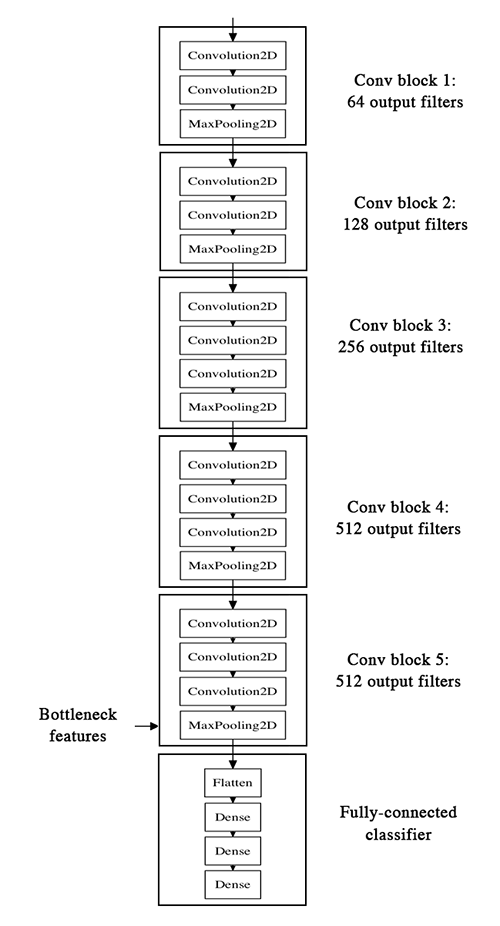
\includegraphics[width=12cm]{pic/assets/pretrained}
    \caption{VGG模型}	\label{VGG模型}	\end{figure}


如图~\ref{vgg16modified}~所示。
\begin{figure}[!htbp]
	\centering	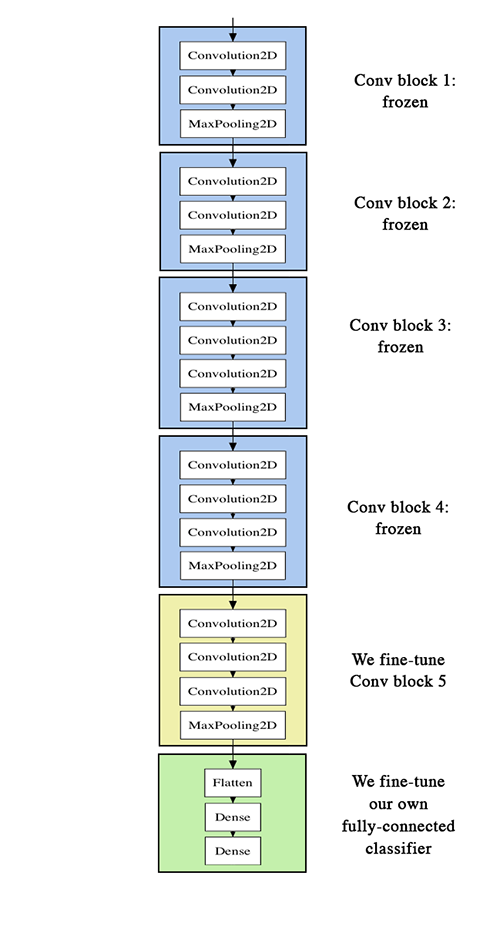
\includegraphics[width=12cm]{pic/assets/vgg16_modified}
    \caption{vgg16 modified}	\label{vgg16modified}	\end{figure}



\subsubsection{模型的训练}

以识别的准确率作为loss,通过keras的model.fit函数在数据集上调整权重,
训练模型。训练的过程保存在history中,
然后我们可以通过后者画出准确率随时间变化的曲线图。

训练任务在我们的笔记本上进行。笔记本没有强大的英伟达显卡,内存也很有限,
因此实验过程还是花了一个多小时。从图中,我们可以看到,由于使用了预训练模型,
一开始起点还是比较高的,但是也很有限,不过要好于从0开始的乱猜,
然后训练中效果提升得很快,当然其中也存在过拟合的情况,
效果提升到一定程度之后,出现瓶颈,在那个点上下波动,
之后有陷入过拟合的趋向,我们停止训练,保存为训练好的模型。

我们的准确度最终已经达到99.3\%,之后可以进行预测了.

\subsection{模型的预测}

模型大致分为两个部分,一是特征提取部分,二是预测部分。
特征提取部分的建立前面已经论述过,这里来谈模型的预测部分。
迁移学习中,迁移之前的预训练和迁移之后的训练,目标并不完全相同,
因此预测层需重新建立。

Resnet50的预训练目标是1000种日常物体多分类(multi-class)问题,
我们的迁移目标是五种自然景物的多标签(multi-label)问题.
这里物体种类的数目(classes)不同,而且问题性质也不同。
实际上很多粗略解决多标签问题的方法都是简单地将其当成多分类问题来解决。
这实际上不是很严谨,但由于训练比较充分,简单地取概率上前几个物体,识别效果还可以。

我们使用的方法是严格地把它作为多标签问题处理.softmax函数适用于multi-class问题,
用在multi-label问题中并不是很恰当,有种祖略的方式是对N个标签,
使用N个softmax函数,这样所有的标签的概率加起来为1。
我们使用的是sigmoid激活函数,这样对于每个标签,都是独立的伯努利分布的概率,
更加符合multi-label任务,经检验也比softmax的识别效果好。

\section{结论和建议}

\subsection{研究成果}
我们通过迁移学习,使预测模型开始就有大概50\%的准确率,将预训练模型抽取的特征很好地
保留下来,通过冻结预训练模型前面多层的权重,有效地避免在小数据集上训练将之前习得的
图像特征给丢失,同时再在特征提取层面添加新层允许权值通过反向传播改变,达到在新任务中
有效提取特征的目的.


\subsection{创新点}

深度学习需要大量的计算资源和资金的支持.若无这些支持,从0开始设计并从头训练一个具有较高性能的
的多标签分类模型基本是不可能的.本次实验实验条件极其有限,我们通过迁移学习,在小数据集上取得了
不错的效果.












% \begin{minted}{c}
%     int main() {
%         printf("hello, world");
%         return 0;
%     }
% \end{minted}



% \clearpage
